%% ============================================================
%%  best_equipo_06: el mejor modelo y la decisión de compra
%%  Plantilla Beamer Uniandes (beamerthemeUniandes.sty, sin cambios).
%%  Compilar con LuaLaTeX:  latexmk -lualatex best_equipo_06.tex
%%  Las cifras y tablas salen de generated/ (scripts/36_build_presentations.py);
%%  las figuras, de ../views/ (scripts 31 a 35). Notas del orador: notas_best.md.
%% ============================================================
\documentclass[aspectratio=169,11pt]{beamer}
%% Preamble: packages and theme. Keep design changes in beamerthemeUniandes.sty
\usepackage[utf8]{inputenc}
\usepackage[T1]{fontenc}
\usepackage[spanish,es-nodecimaldot,es-noshorthands]{babel}
\usepackage{amsmath,amssymb}
\usepackage{graphicx}
\usepackage{booktabs}
\usepackage[round]{natbib}
\usetheme{Uniandes}

\usetikzlibrary{arrows.meta,positioning}
\graphicspath{{../views/}}
% Generado por scripts/36_build_presentations.py a partir de views/. No editar.
\newcommand{\KagBest}{145,7}
\newcommand{\KagPrivate}{148,6}
\newcommand{\RankPublic}{1}
\newcommand{\RankPrivate}{1}
\newcommand{\SharePublic}{20\,\%}
\newcommand{\SharePrivate}{80\,\%}
\newcommand{\KagSecond}{150,8}
\newcommand{\GapSecond}{2,2}
\newcommand{\PrivateRise}{2,9}
\newcommand{\PrivateRisePct}{2,0\,\%}
\newcommand{\GainNaive}{61\,\%}
\newcommand{\KagBoost}{152,1}
\newcommand{\KagNet}{157,1}
\newcommand{\KagLinear}{180,5}
\newcommand{\KagScaled}{171,7}
\newcommand{\KagQsixtyfive}{161,7}
\newcommand{\KagText}{153,1}
\newcommand{\GainText}{7,9}
\newcommand{\GainBetoKaggle}{2,6}
\newcommand{\GainFirst}{216,1}
\newcommand{\GainLast}{15,3}
\newcommand{\GainTotal}{231,4}
\newcommand{\KagStepA}{377,1}
\newcommand{\KagStepB}{180,1}
\newcommand{\KagStepC}{160,9}
\newcommand{\KagStepD}{152,1}
\newcommand{\KagStepE}{148,2}
\newcommand{\KagStepF}{145,7}
\newcommand{\GainStepB}{196,9}
\newcommand{\GainStepC}{19,2}
\newcommand{\GainStepD}{8,9}
\newcommand{\GainStepE}{3,8}
\newcommand{\GainStepF}{2,6}
\newcommand{\MaeBeto}{148,5}
\newcommand{\MaeRidge}{169,1}
\newcommand{\BetoCorr}{0,83}
\newcommand{\BetoTopDecile}{341}
\newcommand{\RidgeTopDecile}{537}
\newcommand{\BetoMidDecile}{133}
\newcommand{\RidgeMidDecile}{87}
\newcommand{\BetoTopBias}{−314}
\newcommand{\RidgeTopBias}{−534}
\newcommand{\SpatialBoostingBefore}{127,0}
\newcommand{\SpatialBoostingAfter}{124,4}
\newcommand{\SpatialRedBefore}{137,6}
\newcommand{\SpatialRedAfter}{133,7}
\newcommand{\SpatialMezclaBefore}{127,6}
\newcommand{\SpatialMezclaAfter}{124,8}
\newcommand{\SpatialBest}{124,8}
\newcommand{\RandomBefore}{95,5}
\newcommand{\TwinsBefore}{112,2}
\newcommand{\RecipeGainMin}{12,3}
\newcommand{\RecipeGainMax}{44,8}
\newcommand{\LinSpatial}{164,1}
\newcommand{\LinNoGeoSpatial}{156,3}
\newcommand{\CorrForest}{0,98}
\newcommand{\CorrNet}{0,96}
\newcommand{\BlendNetGain}{−3,8}
\newcommand{\BlendForestGain}{0,0}
\newcommand{\BlendForestSpatial}{+2,8}
\newcommand{\NNegative}{16}
\newcommand{\MaxNet}{2.002}
\newcommand{\MaxForest}{1.590}
\newcommand{\MaxCart}{1.580}
\newcommand{\OsmSpatial}{+7,9 a +8,6}
\newcommand{\LocalSpatial}{+8,9 a +60,3}
\newcommand{\BalanceSpatial}{−7,7 a +5,5}
\newcommand{\BalanceWeighted}{+0,7 a +4,1}
\newcommand{\StackWeighted}{+15,1 a +23,2}
\newcommand{\SpRandom}{0,44}
\newcommand{\SpTwins}{0,78}
\newcommand{\SpSpatial}{0,74}
\newcommand{\SpWeighted}{0,83}
\newcommand{\GapSpatial}{26,5}
\newcommand{\AsymWinner}{190}
\newcommand{\AsymWinnerQ}{0,20}
\newcommand{\AsymWinnerCost}{174}
\newcommand{\BestCostKthree}{289}
\newcommand{\BestRankKthree}{6}
\newcommand{\BestRankKone}{4}
\newcommand{\NRanked}{13}
\newcommand{\OverClosed}{67\,\%}
\newcommand{\OverCapital}{18\,\%}
\newcommand{\OverMean}{123}
\newcommand{\LowClosed}{33\,\%}
\newcommand{\LowCapital}{12\,\%}
\newcommand{\LowMean}{67}
\newcommand{\SameDiscount}{15\,\%}
\newcommand{\SameClosed}{34\,\%}
\newcommand{\SameCapital}{14\,\%}
\newcommand{\MinCapital}{10\,\%}
\newcommand{\AptClosed}{32\,\%}
\newcommand{\AptCapital}{10,9\,\%}
\newcommand{\HouseCapital}{14,9\,\%}
\newcommand{\ShareOverCheap}{92\,\%}
\newcommand{\ShareOverRich}{18\,\%}
\newcommand{\BiasRich}{−205}
\newcommand{\ShareOverTotal}{67\,\%}
\newcommand{\BiasTotal}{39,4}
\newcommand{\MeanOver}{123,3}
\newcommand{\MeanUnder}{127,9}
\newcommand{\OverHighPred}{204}
\newcommand{\MaeApt}{108,3}
\newcommand{\MaeHouse}{175,7}
\newcommand{\MaeAreaOk}{117,0}
\newcommand{\MaeAreaMissing}{141,7}
\newcommand{\ShareAreaMissing}{26\,\%}
\newcommand{\BiasNortheast}{−53,3}


\title[El mejor modelo y la decisión de compra]{¿Podemos confiar en el modelo para comprar vivienda en Chapinero?}
\subtitle{El mejor modelo y la decisión de compra}
\author[Equipo 06]{[NOMBRES]}
\institute{Big Data y Machine Learning (MECA 4107)\\ Universidad de los Andes}
\date[Nov.\ 2026]{Bogotá, noviembre de 2026}

\newcommand{\twolines}[2]{\begin{tabular}[t]{@{}c@{}}#1\\#2\end{tabular}}
\newcommand{\slidefig}[1]{\centering\includegraphics[width=\textwidth]{#1}\par}

\begin{document}

{\setbeamertemplate{footline}{}
 \begin{frame}[plain,noframenumbering]
   \titlepage
 \end{frame}}

% 1 ---------------------------------------------------------------
\begin{frame}{El modelo predice Chapinero con un error de \KagBest\ millones}
  \vfill
  \begin{columns}[T]
    \column{0.32\textwidth}\centering \keyfig{\KagBest\ M}{MAE público en Kaggle}
    \column{0.32\textwidth}\centering \keyfig{−\GainNaive}{\twolines{frente a predecir la mediana}{(\KagNaive\ M)}}
    \column{0.32\textwidth}\centering \keyfig{\SpatialBest\ M}{\twolines{MAE en zonas que no vio}{(validación espacial)}}
  \end{columns}
  \vfill
  \begin{center}\small
    \begin{tabular}{lrr}
      \toprule
      Si la empresa ofrece\ldots & Compra & Sobrepago / capital \\
      \midrule
      lo que predice el modelo   & \OverClosed & \OverCapital \\
      el cuantil 0,20 del precio & \LowClosed  & \LowCapital \\
      \bottomrule
    \end{tabular}
  \end{center}
  \vfill
  \takeaway{Sirve para escoger candidatos, no para fijar el precio de compra.}
\end{frame}

% 2 ---------------------------------------------------------------
\begin{frame}{Entrenamos en el resto de Bogotá; Chapinero es más caro}
  \begin{columns}[c]
    \column{0.47\textwidth}
      \centering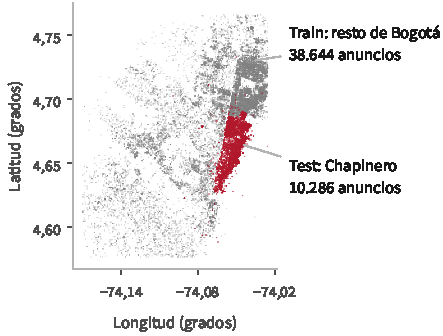
\includegraphics[width=\linewidth]{map_train_test}
    \column{0.51\textwidth}
      \centering\footnotesize
      % Generado por scripts/36_build_presentations.py. No editar.
\begin{tabular}{lrr}
\toprule
 & Resto de Bogotá & Chapinero \\
\midrule
Casas (\%) & 24 & 3 \\
Área (m², mediana) & 112 & 119 \\
Alcobas (media) & 3,1 & 2,4 \\
Estrato (media) & 4,6 & 5,4 \\
Terreno (mil \$/m²) & 3.200 & 6.000 \\
Sin área en el anuncio (\%) & 39 & 36 \\
\bottomrule
\end{tabular}

  \end{columns}
  \takeaway{Chapinero casi no tiene casas y su terreno vale \LandRatio\ veces más.}
\end{frame}

% 3 ---------------------------------------------------------------
\begin{frame}{El modelo: un boosting y una red neuronal que apuntan alto}
  \centering
  \begin{tikzpicture}[
      font=\footnotesize, align=center, line width=0.4pt,
      box/.style={draw=andesmid, rounded corners=2pt, inner sep=4pt,
                  minimum height=1.05cm, text width=3.6cm},
      head/.style={font=\scriptsize\bfseries, text=andesgray},
      flow/.style={-{Stealth[length=4pt,width=3pt]}, draw=andesgray, line width=0.5pt}]
    % Columna 1: qué ve el modelo
    \node[box] (struct) at (0, 1.35) {\textbf{El inmueble}\\tipo, alcobas, baños, área};
    \node[box] (place)  at (0, 0)    {\textbf{La ubicación}\\estrato, terreno, distancias};
    \node[box] (text)   at (0,-1.35) {\textbf{El texto del anuncio}\\18 señales y un ridge};
    % Columna 2: los dos modelos
    \node[box, draw=andesaccent, line width=0.8pt] (boost) at (4.95, 0.75)
         {\textbf{Boosting cuantílico}\\cuantil 0,70 del precio\\peso 70\,\%};
    \node[box, draw=andesred, line width=0.8pt] (net) at (4.95,-0.75)
         {\textbf{Red neuronal cuantílica}\\cuantil 0,70 del precio\\peso 30\,\%};
    % Columna 3: la predicción
    \node[box, draw=andesblack, line width=0.8pt] (pred) at (9.85, 0)
         {\textbf{Precio de oferta}\\0,7 boosting + 0,3 red\\millones de pesos};
    % Encabezados alineados
    \node[head] at (0, 2.35)    {Qué ve el modelo};
    \node[head] at (4.95, 2.35)  {Dos modelos por tipo de inmueble};
    \node[head] at (9.85, 2.35) {La predicción};
    % Flechas: las tres entradas se juntan y alimentan los dos modelos
    \coordinate (join) at (2.65, 0);
    \foreach \src in {struct, place, text}
      \draw[draw=andesgray, line width=0.5pt] (\src.east) -- (2.35, 0 |- \src.east) -- (join);
    \draw[flow] (join) |- (boost.west);
    \draw[flow] (join) |- (net.west);
    \draw[flow] (boost.east) -- (pred.west);
    \draw[flow] (net.east) -- (pred.west);
  \end{tikzpicture}
  \par\vspace{0.35cm}
  \begin{minipage}{0.92\textwidth}\small\raggedright
    Los dos apuntan al cuantil 0,70 porque Chapinero es más caro que el resto de Bogotá.
    La red puede predecir por encima del tope de 1.650 M que limita a los árboles.
  \end{minipage}
\end{frame}

% 4 ---------------------------------------------------------------
\begin{frame}{Cada mejora en Kaggle tiene una causa}
  \slidefig{kaggle_progression}
  \takeaway{La mezcla con la red le gana \GainBoost\ M al mejor boosting solo (\KagBoost\ M).}
\end{frame}

% 5 ---------------------------------------------------------------
\begin{frame}{El texto del anuncio es lo que más pesa en el modelo}
  \slidefig{best_errors_importance}
  \takeaway{El ridge sobre el texto aporta el \ImpApt\ de la ganancia en apartamentos.}
\end{frame}

% 6 ---------------------------------------------------------------
\begin{frame}{El modelo sobrepredice los baratos y subpredice los caros}
  \slidefig{best_errors_segments}
  \takeaway{Sobrepredice el \ShareOverCheap\ de los de menos de 400 M y el \ShareOverRich\ de los de más de 1.200 M.}
\end{frame}

% 7 ---------------------------------------------------------------
\begin{frame}{Si pagar de más cuesta el triple, gana el cuantil \AsymWinnerQ}
  \slidefig{asymmetric_ranking}
  \takeaway{La mezcla que gana en Kaggle cae al puesto \BestRankKthree\ cuando pagar de más cuesta el triple.}
\end{frame}

% 8 ---------------------------------------------------------------
\begin{frame}{Ofrecer la predicción compra justo lo que sobreestima}
  \slidefig{purchase_rule_frontier}
  \takeaway{A igual número de compras, bajar el cuantil sobrepaga menos que dar un descuento.}
\end{frame}

% 9 ---------------------------------------------------------------
\begin{frame}{Proponemos el cuantil 0,20, solo en apartamentos}
  \vfill
  \centering\footnotesize
  % Generado por scripts/36_build_presentations.py. No editar.
\begin{tabular}{llrrr}
\toprule
Regla & Segmento & Compras & Sobrepago medio & Sobrepago / capital \\
\midrule
Mezcla 203 (q0,70) & Todos & 67\,\% & 123 & 18,0\,\% \\
Cuantil 0,20 & Todos & 33\,\% & 67 & 12,1\,\% \\
\textbf{Cuantil 0,20} & \textbf{Apartamentos con área} & \textbf{33\,\%} & \textbf{59} & \textbf{10,8\,\%} \\
\textbf{Cuantil 0,20} & \textbf{Apartamentos sin área} & \textbf{30\,\%} & \textbf{54} & \textbf{11,4\,\%} \\
Cuantil 0,20 & Casas con área & 36\,\% & 98 & 15,1\,\% \\
Cuantil 0,20 & Casas sin área & 32\,\% & 83 & 14,4\,\% \\
\bottomrule
\end{tabular}

  \par\vspace{4pt}{\scriptsize\color{andesgray} Validación espacial fuera de muestra; sobrepago frente al precio pedido.}
  \vfill
  \takeaway{En apartamentos el sobrepago es \AptCapital\ del capital; en casas, \HouseCapital.}
\end{frame}

% 10 --------------------------------------------------------------
\begin{frame}{Para escoger candidatos sí; para fijar el precio, no}
  \begin{itemize}
    \item Usar el cuantil 0,20 sin descuento para escoger candidatos.
    \item Solo apartamentos; cerrar después de una tasación física.
    \item No usarlo en casas ni con predicciones de más de 900 M.
  \end{itemize}
  \vfill
  \begin{columns}[T]
    \column{0.45\textwidth}\centering \keyfig{\AptClosed}{\twolines{de los apartamentos se compran}{con el cuantil 0,20}}
    \column{0.45\textwidth}\centering \keyfig{\AptCapital}{\twolines{de sobrepago sobre el capital, frente a}{\OverCapitalD\ con el modelo de Kaggle}}
  \end{columns}
  \vfill
  \takeaway{Antes de comprometer capital, revisar la regla con precios de cierre.}
\end{frame}

% 11 --------------------------------------------------------------
\begin{frame}{Cuatro riesgos pueden subir el sobrepago real}
  \begin{itemize}
    \item \textbf{Precios de oferta, no de cierre:} si se vende por menos, se pagó de más.
    \item \textbf{Área faltante} en el \ShareAreaMissing\ de los anuncios: el MAE sube de \MaeAreaOk\ a \MaeAreaMissing\ M.
    \item \textbf{Datos de 2019 a 2021:} el mercado pudo cambiar.
    \item \textbf{Cambio de zona:} la espacial da \SpatialBest\ M y Kaggle \KagBest\ M; el nivel en Chapinero es incierto.
  \end{itemize}
  \takeaway{El modelo filtra; la tasación decide.}
\end{frame}

\andesclosing{¡Gracias!}{Equipo 06 · MECA 4107}

\end{document}
